\documentclass{article}
\usepackage{fancyhdr}
\usepackage{ctex}
\usepackage{listings}
\usepackage{graphicx}
\usepackage[a4paper, body={18cm,22cm}]{geometry}
\usepackage{amsmath,amssymb,amstext,wasysym,enumerate,graphicx}
\usepackage{float,abstract,booktabs,indentfirst,amsmath}
\usepackage{array}
\usepackage{booktabs}
\usepackage{multirow}
\usepackage{url}
\usepackage{diagbox}
\renewcommand\arraystretch{1.4}
\usepackage{indentfirst}
\setlength{\parindent}{2em}
\usepackage{enumitem}
\setmonofont{JetBrains Mono}
\usepackage{listings}
\usepackage{xcolor}
\usepackage{makecell}
\usepackage{tikz}
\usepackage{subfig}
\usetikzlibrary{positioning, arrows.meta}
\setCJKmonofont{黑体}
\lstset{
    % language = C,
    xleftmargin = 3em,xrightmargin = 3em, aboveskip = 1em,
	backgroundcolor = \color{white}, % 背景色
	basicstyle = \small\ttfamily, % 基本样式 + 小号字体
	rulesepcolor= \color{gray}, % 代码块边框颜色
	breaklines = true, % 代码过长则换行
	numbers = left, % 行号在左侧显示
	numberstyle = \small, % 行号字体
    numbersep = -14pt, 
    keywordstyle=\color{purple}\bfseries, % 关键字颜色
    commentstyle =\color{red!50!green!50!blue!60}, % 注释颜色
    stringstyle = \color{red!60!green!90!blue!90}, % 字符串颜色
    morekeywords={ASSERT, int64_t, uint32_t},
	frame = shadowbox, % 用(带影子效果)方框框住代码块
	showspaces = false, % 不显示空格
	columns = fixed, % 字间距固定
} 
\lstset{
    sensitive=true,
    moreemph={ASSERT, NULL}, emphstyle=\color{red}\bfseries,
    moreemph=[2]{int64_t, uint32_t, tid_t, uint8_t, int16_t, uint16_t, int32_t, size_t, bool}, emphstyle=[2]\color{purple}\bfseries,
    commentstyle=\color{green!60!black}, % 设置注释颜色
    morecomment=[l][\color{green!60!black}]{+}, % 设置以+开头的代码行为绿色
}
%--------------------页眉--------------------%
\pagestyle{fancy}
\fancyhead[L]{}
\fancyhead[R]{}
\fancyhead[C]{华东师范大学软件工程学院实验报告}
\fancyfoot[C]{-\thepage-}
\renewcommand{\headrulewidth}{1.5pt}
%--------------------标题--------------------%
\begin{document}
\begin{center}
  {\Large{\textbf{\heiti 华东师范大学软件工程学院实验报告}}}
  \begin{table}[H]
    \centering
    \begin{tabular}{p{2cm}p{4cm}<{\centering}p{1cm}p{2cm}p{6cm}<{\centering}}
      姓\qquad 名: & 李鹏达    & \quad & 学\qquad 号: & 10225101460               \\ \cline{2-2} \cline{5-5}
      实验编号:    & Project 2 & \quad & 实验名称:    & {User Programs in Pintos}
      \\ \cline{2-2} \cline{5-5}
    \end{tabular}
  \end{table}
\end{center}
\rule{\textwidth}{1pt}
%--------------------正文--------------------%
\section{实验目的}

\begin{enumerate}[noitemsep, label={{\arabic*})}]
  \item 实现参数传递
  \item 实现系统调用
\end{enumerate}
\normalsize
\section{实验内容与实验步骤}

为防止之前的 Project1 可能存在的 bug对本次实验造成影响,我们从未完成 Project1 的代码开始,进行本次实验的实现。

首先,我们将 \texttt{src/utils} 中的 \texttt{pintos} 和 \texttt{Pintos.pm} 中对应的 \texttt{src/threads} 改为 \texttt{src/userprog}。


\subsection{参数传递}

首先,我们需要再线程结构体中添加 \texttt{struct semaphore sema} 和 \texttt{struct thread* parent},分别用于实现进程的同步和父进程的记录,以及 \texttt{bool success},用于记录进程是否成功加载。

\begin{lstlisting}[language=C, title={\texttt{src/threads/thread.h}}]
    struct thread
      {
        /* Owned by thread.c. */
        tid_t tid;                          /* Thread identifier. */
        enum thread_status status;          /* Thread state. */
        char name[16];                      /* Name (for debugging purposes). */
        uint8_t *stack;                     /* Saved stack pointer. */
        int priority;                       /* Priority. */
        struct list_elem allelem;           /* List element for all threads list. */

        /* Shared between thread.c and synch.c. */
        struct list_elem elem;              /* List element. */

    #ifdef USERPROG
        /* Owned by userprog/process.c. */
        uint32_t *pagedir;                  /* Page directory. */
        struct semaphore sema;
        struct thread* parent;
        bool success;
    #endif

        /* Owned by thread.c. */
        unsigned magic;                     /* Detects stack overflow. */
      };
\end{lstlisting}

然后在线程的初始化函数 \texttt{thread\_init()}中,对这些变量进行初始化。

\begin{lstlisting}[language=C, title={\texttt{src/threads/thread.c}}]
    static void
    init_thread (struct thread *t, const char *name, int priority)
    {
      enum intr_level old_level;
    
      ASSERT (t != NULL);
      ASSERT (PRI_MIN <= priority && priority <= PRI_MAX);
      ASSERT (name != NULL);
    
      memset (t, 0, sizeof *t);
      t->status = THREAD_BLOCKED;
      strlcpy (t->name, name, sizeof t->name);
      t->stack = (uint8_t *) t + PGSIZE;
      t->priority = priority;
      t->magic = THREAD_MAGIC;
    
    #ifdef USERPROG
      if (t == initial_thread)
        t->parent = NULL;
      else
        t->parent = thread_current ();
      sema_init (&t->sema, 0);
      t->success = true;
    #endif
    
      old_level = intr_disable ();
      list_push_back (&all_list, &t->allelem);
      intr_set_level (old_level);
    }

\end{lstlisting}

接下来,我们需要修改 \texttt{src/userprog/process.c} 中的 \texttt{process\_execute()}函数,使得其能够将参数传递给新的进程。

\begin{lstlisting}[language=C, title=\texttt{src/userprog/process.c - process\_execute()}]
    process_execute (const char *file_name) 
    {
      char *fn_copy;
      char *fn_copy2;
      char *save_ptr;
      char *token;
      tid_t tid;
    
      /* Make a copy of FILE_NAME.
        Otherwise there's a race between the caller and load(). */
      fn_copy = palloc_get_page (0);
      if (fn_copy == NULL)
        return TID_ERROR;
      fn_copy2 = palloc_get_page (0);
      if (fn_copy2 == NULL)
      {
        palloc_free_page(fn_copy);
        return TID_ERROR;
      }
    
      strlcpy (fn_copy, file_name, PGSIZE);
      strlcpy (fn_copy2, file_name, PGSIZE);
    
      token = strtok_r (fn_copy, " ", &save_ptr);
    
      /* Create a new thread to execute FILE_NAME. */
      tid = thread_create (token, PRI_DEFAULT, start_process, fn_copy2);
      palloc_free_page(fn_copy);
      if (tid == TID_ERROR)
      {
        palloc_free_page (fn_copy2); 
        return tid;
      }
      sema_down(&thread_current ()->sema);
      if (!thread_current ()->success)
        return TID_ERROR;
      return tid;
    }
\end{lstlisting}

在 \texttt{process\_execute()}中,我们首先将 \texttt{file\_name}复制到 \texttt{fn\_copy}和 \texttt{fn\_copy2}中,然后使用 \texttt{strtok\_r()}函数将 \texttt{fn\_copy}中的字符串按照空格分割,得到第一个参数,即可执行的程序名。然后,我们调用 \texttt{thread\_create()}函数创建一个新的线程,将第一个参数作为线程的名字,将 \texttt{fn\_copy2}作为线程的参数,将 \texttt{start\_process}作为线程的执行函数。最后,我们调用 \texttt{sema\_down()}函数,使得父进程等待子进程执行完毕,然后再返回。

接下来,我们需要修改 \texttt{src/userprog/process.c} 中的 \texttt{start\_process()}函数,使得其能够将参数压入栈中。

为此,我们定义一个 \texttt{push\_args()} 函数,用于将参数压入栈中。

其中压入参数的顺序和结构如图所示:

\begin{figure}[H]
  \centering
  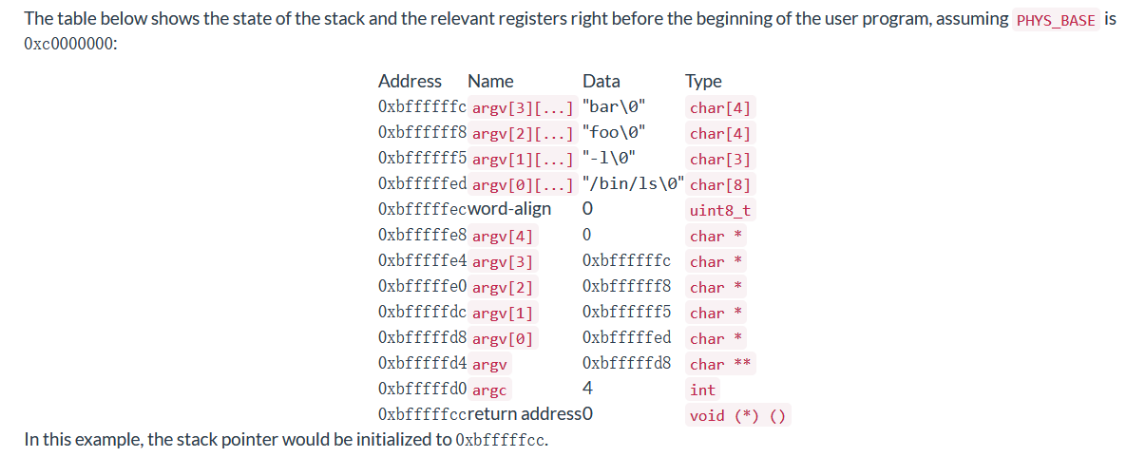
\includegraphics[width=0.9\textwidth]{img/1.png}
  \caption{压入参数的顺序和结构}
\end{figure}

\begin{lstlisting}[language=C, title=\texttt{src/userprog/process.c - push\_args()}]
    static void
    push_args(void **esp, int argc, char* argv[])
    {
      int i;
      *esp = (void *)((int)*esp & 0xfffffffc);
      *esp -= 4;
      *(uint32_t *) *esp = 0;
      for (i = argc - 1; i >= 0; i--)
      {
        *esp -= 4;
        *(uint32_t *) *esp = (uint32_t)argv[i];
      }
      *esp -= 4;
      *(uint32_t *) *esp = (uint32_t)*esp + 4;
      *esp -= 4;
      *(uint32_t *) *esp = argc;
      *esp -= 4;
      *(uint32_t *) *esp = 0;
    }
\end{lstlisting}

在 \texttt{start\_process()}函数中,我们首先将参数 \texttt{file\_name}复制到 \texttt{fn\_copy}中,然后使用 \texttt{strtok\_r()}函数将 \texttt{fn\_copy}中的字符串按照空格分割,得到第一个参数,即可执行的程序名。然后,调用 \texttt{load()}函数加载程序,如果加载成功,则将参数压入栈中,然后唤醒父进程,否则,唤醒父进程并退出。

\begin{lstlisting}[language=C, title=\texttt{src/userprog/process.c - start\_process()}]
    static void
    start_process (void *file_name_)
    {
      char *file_name = file_name_;
      char *fn_copy;
      char *save_ptr;
      char *token;
      struct intr_frame if_;
      bool success;
      int argc = 0;
      char *argv[50];
    
      fn_copy = malloc (strlen (file_name) + 1);
      strlcpy (fn_copy, file_name, strlen (file_name) + 1);
    
      /* Initialize interrupt frame and load executable. */
      memset (&if_, 0, sizeof if_);
      if_.gs = if_.fs = if_.es = if_.ds = if_.ss = SEL_UDSEG;
      if_.cs = SEL_UCSEG;
      if_.eflags = FLAG_IF | FLAG_MBS;
    
      file_name = strtok_r (file_name, " ", &save_ptr);
      success = load (file_name, &if_.eip, &if_.esp);
    
      if (success)
      {
        for (token = strtok_r (fn_copy, " ", &save_ptr); token != NULL; token = strtok_r (NULL, " ", &save_ptr))
        {
          if_.esp -= (strlen(token) + 1);
          memcpy (if_.esp, token, strlen(token) + 1);
          argv[argc++] = (char *)if_.esp;
        }
        push_args (&if_.esp, argc, argv);
        thread_current ()->parent->success = true;
        sema_up(&thread_current ()->parent->sema);
      }
    
      /* If load failed, quit. */
      palloc_free_page (file_name);
      free (fn_copy);
      if (!success)
      {
        thread_current()->parent->success = false;
        sema_up(&thread_current ()->parent->sema);
        thread_exit ();
      }
    
      /* Start the user process by simulating a return from an
        interrupt, implemented by intr_exit (in
        threads/intr-stubs.S).  Because intr_exit takes all of its
        arguments on the stack in the form of a `struct intr_frame',
        we just point the stack pointer (%esp) to our stack frame
        and jump to it. */
      asm volatile ("movl %0, %%esp; jmp intr_exit" : : "g" (&if_) : "memory");
      NOT_REACHED ();
    }

\end{lstlisting}

到这里,参数传递的实现就完成了。我们可以尝试运行一个测试用例:

\begin{lstlisting}[language=, title=测试用例]
    $ pintos -v -k -T 60 --qemu  --filesys-size=2 -p build/tests/userprog/args-none -a args-none -- -q  -f run args-none
    SeaBIOS (version 1.15.0-1)
    Booting from Hard Disk...
    PPiiLLoo  hhddaa1
    1
    LLooaaddiinngg.......................
    Kernel command line: -q -f extract run 'args-single onearg'
    Pintos booting with 3,968 kB RAM...
    367 pages available in kernel pool.
    367 pages available in user pool.
    Calibrating timer...  556,236,800 loops/s.
    ide0: unexpected interrupt
    hda: 5,040 sectors (2 MB), model "QM00001", serial "QEMU HARDDISK"
    hda1: 195 sectors (97 kB), Pintos OS kernel (20)
    hda2: 4,096 sectors (2 MB), Pintos file system (21)
    hda3: 117 sectors (58 kB), Pintos scratch (22)
    ide1: unexpected interrupt
    filesys: using hda2
    scratch: using hda3
    Formatting file system...done.
    Boot complete.
    Extracting ustar archive from scratch device into file system...
    Putting 'args-single' into the file system...
    Erasing ustar archive...
    Executing 'args-single onearg':
    system call!
    Execution of 'args-single onearg' complete.
    Timer: 71 ticks
    Thread: 8 idle ticks, 63 kernel ticks, 0 user ticks
    hda2 (filesys): 63 reads, 238 writes
    hda3 (scratch): 116 reads, 2 writes
    Console: 930 characters output
    Keyboard: 0 keys pressed
    Exception: 0 page faults
    Powering off...
\end{lstlisting}

发现输出了 \texttt{system call!},这是由于我们没有实现相关的系统调用。

\subsection{系统调用}

首先,我们需要在 \texttt{src/userprog/syscall.c} 建议一个指针数组 \texttt{syscall\_table},用于存放系统调用的函数指针。

\begin{lstlisting}[language=C, title=\texttt{src/userprog/syscall.c}]
    #include <syscall-nr.h>

    #define MAX_SYSCALL (SYS_INUMBER)
    
    typedef void (*syscall_func) (struct intr_frame *);
    
    static void syscall_handler (struct intr_frame *);
    static syscall_func syscall_table[MAX_SYSCALL + 1];
\end{lstlisting}

接着,我们定义相关的系统调用函数。

\begin{lstlisting}[language=C, title=\texttt{src/userprog/syscall.h}]
    void syscall_halt (struct intr_frame *f);
    void syscall_exit (struct intr_frame *f);
    void syscall_exec (struct intr_frame *f);
    void syscall_wait (struct intr_frame *f);
    
    void syscall_create (struct intr_frame *f);
    void syscall_remove (struct intr_frame *f);
    void syscall_open (struct intr_frame *f);
    void syscall_filesize (struct intr_frame *f);
    void syscall_read (struct intr_frame *f);
    void syscall_write (struct intr_frame *f);
    void syscall_seek (struct intr_frame *f);
    void syscall_tell (struct intr_frame *f);
    void syscall_close (struct intr_frame *f);
\end{lstlisting}

然后,我们需要在 \texttt{syscall\_init()}函数中初始化 \texttt{syscall\_table}。

\begin{lstlisting}[language=C, title=\texttt{src/userprog/syscall.c - syscall\_init()}]
    void
    syscall_init (void) 
    {
      intr_register_int (0x30, 3, INTR_ON, syscall_handler, "syscall");
      syscall_table[SYS_HALT] = syscall_halt;
      syscall_table[SYS_EXIT] = syscall_exit;
      syscall_table[SYS_EXEC] = syscall_exec;
      syscall_table[SYS_WAIT] = syscall_wait;
      syscall_table[SYS_CREATE] = syscall_create;
      syscall_table[SYS_REMOVE] = syscall_remove;
      syscall_table[SYS_OPEN] = syscall_open;
      syscall_table[SYS_FILESIZE] = syscall_filesize;
      syscall_table[SYS_READ] = syscall_read;
      syscall_table[SYS_WRITE] = syscall_write;
      syscall_table[SYS_SEEK] = syscall_seek;
      syscall_table[SYS_TELL] = syscall_tell;
      syscall_table[SYS_CLOSE] = syscall_close;
    }
\end{lstlisting}

在进行系统调用时,我们需要访问用户空间的内存,因此,我们需要实现 \texttt{get\_user()}函数和 \texttt{check\_ptr()}函数,用于检验用户空间的内存是否合法。在内存不合法时,我们定义一个 \texttt{exit\_error()}函数,用于退出进程,并返回 \texttt{-1}。

\begin{lstlisting}[language=C, title=\texttt{src/userprog/syscall.c - get\_user()}]
    static int
    get_user (const uint8_t *uaddr)
    {
      int result;
      asm ("movl $1f, %0; movzbl %1, %0; 1:"
            : "=&a" (result) : "m" (*uaddr));
      return result;
    }
\end{lstlisting}

\begin{lstlisting}[language=C, title=\texttt{src/userprog/syscall.c - check\_ptr()}]
    static void *
    check_ptr (const void *vaddr)
    {
      if (!is_user_vaddr (vaddr))
        exit_error ();
      void *ptr = pagedir_get_page (thread_current ()->pagedir, vaddr);
      if (!ptr)
        exit_error ();
      uint8_t *uaddr = (uint8_t *) vaddr;
      for (; uaddr < (uint8_t *) vaddr + sizeof (int); uaddr++)
        if (get_user (uaddr) == -1)
          exit_error ();
      return ptr;
    }
\end{lstlisting}

\begin{lstlisting}[language=C, title=\texttt{src/userprog/syscall.c - exit\_error()}]
    static void
    exit_error (void)
    {
      thread_current ()->exit_status = -1;
      thread_exit ();
    }
\end{lstlisting}

在这里,为了存储线程的退出状态,我们需要在线程结构体中添加 \texttt{int exit\_status}。

\begin{lstlisting}[language=C, title=\texttt{src/threads/thread.h}]
    struct thread
      {
        /* Owned by thread.c. */
        tid_t tid;                          /* Thread identifier. */
        enum thread_status status;          /* Thread state. */
        char name[16];                      /* Name (for debugging purposes). */
        uint8_t *stack;                     /* Saved stack pointer. */
        int priority;                       /* Priority. */
        struct list_elem allelem;           /* List element for all threads list. */

        /* Shared between thread.c and synch.c. */
        struct list_elem elem;              /* List element. */

    #ifdef USERPROG
        /* Owned by userprog/process.c. */
        uint32_t *pagedir;                  /* Page directory. */
        struct semaphore sema;
        struct thread* parent;
        bool success;
        int exit_status;
    #endif

        /* Owned by thread.c. */
        unsigned magic;                     /* Detects stack overflow. */
      };
\end{lstlisting}

接下来,修改 \texttt{page\_fault()}函数,使得其能够处理用户空间的内存错误。

\begin{lstlisting}[language=C, title=\texttt{src/userprog/exception.c - page\_fault()}]
    static void
    page_fault (struct intr_frame *f) 
    {
      bool not_present;  /* True: not-present page, false: writing r/o page. */
      bool write;        /* True: access was write, false: access was read. */
      bool user;         /* True: access by user, false: access by kernel. */
      void *fault_addr;  /* Fault address. */
    
      /* Obtain faulting address, the virtual address that was
        accessed to cause the fault.  It may point to code or to
        data.  It is not necessarily the address of the instruction
        that caused the fault (that's f->eip).
        See [IA32-v2a] "MOV--Move to/from Control Registers" and
        [IA32-v3a] 5.15 "Interrupt 14--Page Fault Exception
        (#PF)". */
      asm ("movl %%cr2, %0" : "=r" (fault_addr));
    
      /* Turn interrupts back on (they were only off so that we could
        be assured of reading CR2 before it changed). */
      intr_enable ();
    
      /* Count page faults. */
      page_fault_cnt++;
    
      /* Determine cause. */
      not_present = (f->error_code & PF_P) == 0;
      write = (f->error_code & PF_W) != 0;
      user = (f->error_code & PF_U) != 0;
    
      if (!user)
      {
        f->eip = (void (*) (void)) f->eax;
        f->eax = UINT32_MAX;
        return;
      }
    
      /* To implement virtual memory, delete the rest of the function
        body, and replace it with code that brings in the page to
        which fault_addr refers. */
      printf ("Page fault at %p: %s error %s page in %s context.\n",
              fault_addr,
              not_present ? "not present" : "rights violation",
              write ? "writing" : "reading",
              user ? "user" : "kernel");
      kill (f);
    }
\end{lstlisting}

然后,我们需要实现 \texttt{syscall\_handler()}函数,用于处理系统调用。

\begin{lstlisting}[language=C, title=\texttt{src/userprog/syscall.c - syscall\_handler()}]
    static void
    syscall_handler (struct intr_frame *f UNUSED) 
    {
      check_ptr ((int *)f->esp + 1);
      int syscall_num = *(int *) f->esp;
      if (syscall_num < 0 || syscall_num > MAX_SYSCALL)
        exit_error ();
      syscall_table[syscall_num] (f);
    }
\end{lstlisting}

接下来,我们实现相关的系统调用函数。

\subsubsection{\texttt{halt()}}

\texttt{halt()}函数用于关闭系统。

\begin{lstlisting}[language=C, title=\texttt{src/userprog/syscall.c - syscall\_halt()}]
    void
    syscall_halt (struct intr_frame *f UNUSED)
    {
      shutdown_power_off ();
    }
\end{lstlisting}

\subsubsection{\texttt{exit()}}

\texttt{exit()}函数用于退出进程。

\begin{lstlisting}[language=C, title=\texttt{src/userprog/syscall.c - syscall\_exit()}]
    void
    syscall_exit (struct intr_frame *f)
    {
      check_ptr ((uint32_t *)f->esp + 1);
      int status = *(int *)((uint32_t *)f->esp + 1);
      thread_current ()->exit_status = status;
      thread_exit ();
    }
\end{lstlisting}

\subsubsection{\texttt{exec()}}

\texttt{exec()}函数用于执行程序。

\begin{lstlisting}[language=C, title=\texttt{src/userprog/syscall.c - syscall\_exec()}]
    void
    syscall_exec (struct intr_frame *f)
    {
      check_ptr ((int *)f->esp + 1);
      char *cmd_line = *(char **)(f->esp + 4);
      check_ptr (cmd_line);
      f->eax = process_execute (cmd_line);
    }
\end{lstlisting}

\subsubsection{\texttt{wait()}}

\texttt{wait()}函数用于等待子进程执行完毕。

\begin{lstlisting}[language=C, title=\texttt{src/userprog/syscall.c - syscall\_wait()}]
    void
    syscall_wait (struct intr_frame *f)
    {
      check_ptr ((int *)f->esp + 1);
      tid_t tid = *(tid_t *)(f->esp + 4);
      f->eax = process_wait (tid);
    }
\end{lstlisting}

然后,我们需要修改 \texttt{src/userprog/process.c} 中的 \texttt{process\_wait()}函数,使得其能够等待子进程执行完毕。

首先,我们需要修改线程结构体,添加 \texttt{struct list children},用于存放子进程的线程结构体,以及定义子线程结构体 \texttt{struct child},用于存放子进程的信息。同时,我们需要在线程结构体中添加 \texttt{struct child * child\_thread},用于记录当前线程的子线程结构体。

\begin{lstlisting}[language=C, title=\texttt{src/threads/thread.h}]
    struct thread
      {
        /* Owned by thread.c. */
        tid_t tid;                          /* Thread identifier. */
        enum thread_status status;          /* Thread state. */
        char name[16];                      /* Name (for debugging purposes). */
        uint8_t *stack;                     /* Saved stack pointer. */
        int priority;                       /* Priority. */
        struct list_elem allelem;           /* List element for all threads list. */

        /* Shared between thread.c and synch.c. */
        struct list_elem elem;              /* List element. */

    #ifdef USERPROG
        /* Owned by userprog/process.c. */
        uint32_t *pagedir;                  /* Page directory. */
        struct semaphore sema;
        struct thread* parent;
        bool success;
        int exit_status;
        struct list children;
        struct clild *child_thread;
    #endif

        /* Owned by thread.c. */
        unsigned magic;                     /* Detects stack overflow. */
      };

    #ifdef USERPROG
    struct child
    {
      tid_t tid;
      int exit_status;
      bool running;
      struct semaphore sema;
      struct list_elem elem;
    };
    #endif

\end{lstlisting}

接下来,修改 \texttt{create\_thread()}函数,和 \texttt{init\_thread()}函数,使得其能够初始化这些量。

\begin{lstlisting}[language=C, title=\texttt{src/threads/thread.c - create\_thread()}]
    tid_t
    thread_create (const char *name, int priority,
                  thread_func *function, void *aux) 
    {
      struct thread *t;
      struct kernel_thread_frame *kf;
      struct switch_entry_frame *ef;
      struct switch_threads_frame *sf;
      tid_t tid;
    
      ASSERT (function != NULL);
    
      /* Allocate thread. */
      t = palloc_get_page (PAL_ZERO);
      if (t == NULL)
        return TID_ERROR;
    
      /* Initialize thread. */
      init_thread (t, name, priority);
      tid = t->tid = allocate_tid ();
    #ifdef USERPROG
      struct child *c = malloc (sizeof (struct child));
      c->tid = tid;
      sema_init (&c->sema, 0);
      list_push_back (&thread_current ()->children, &c->elem);
      c->exit_status = UINT32_MAX;
      c->running = false;
      t->child_thread = c;
    #endif
    
      /* Stack frame for kernel_thread(). */
      kf = alloc_frame (t, sizeof *kf);
      kf->eip = NULL;
      kf->function = function;
      kf->aux = aux;
    
      /* Stack frame for switch_entry(). */
      ef = alloc_frame (t, sizeof *ef);
      ef->eip = (void (*) (void)) kernel_thread;
    
      /* Stack frame for switch_threads(). */
      sf = alloc_frame (t, sizeof *sf);
      sf->eip = switch_entry;
      sf->ebp = 0;
    
      /* Add to run queue. */
      thread_unblock (t);
    
      return tid;
    }
\end{lstlisting}

\begin{lstlisting}[language=C, title=\texttt{src/threads/thread.c - init\_thread()}]
    static void
    init_thread (struct thread *t, const char *name, int priority)
    {
      enum intr_level old_level;
    
      ASSERT (t != NULL);
      ASSERT (PRI_MIN <= priority && priority <= PRI_MAX);
      ASSERT (name != NULL);
    
      memset (t, 0, sizeof *t);
      t->status = THREAD_BLOCKED;
      strlcpy (t->name, name, sizeof t->name);
      t->stack = (uint8_t *) t + PGSIZE;
      t->priority = priority;
      t->magic = THREAD_MAGIC;
    
    #ifdef USERPROG
      if (t == initial_thread)
        t->parent = NULL;
      else
        t->parent = thread_current ();
      list_init (&t->children);
      sema_init (&t->sema, 0);
      t->success = true;
      t->exit_status = UINT32_MAX;
    #endif
    
      old_level = intr_disable ();
      list_push_back (&all_list, &t->allelem);
      intr_set_level (old_level);
    }
\end{lstlisting}

然后,我们需要修改 \texttt{process\_wait()}函数。

\begin{lstlisting}[language=C, title=\texttt{src/userprog/process.c - process\_wait()}]
    int
    process_wait (tid_t child_tid UNUSED) 
    {
      struct list *l = &thread_current ()->children;
      struct list_elem *child_elem_ptr;
      child_elem_ptr = list_begin (l);
      struct child *child_ptr = NULL;
      while (child_elem_ptr != list_end (l))
      {
        child_ptr = list_entry (child_elem_ptr, struct child, elem);
        if (child_ptr->tid == child_tid)
        {
          if (!child_ptr->running)
          {
            child_ptr->running = true;
            sema_down (&child_ptr->sema);
            break;
          } 
          else 
            return -1;
        }
        child_elem_ptr = list_next (child_elem_ptr);
      }
      if (child_elem_ptr == list_end (l))
        return -1;
      list_remove (child_elem_ptr);
      return child_ptr->exit_status;
  }
\end{lstlisting}

在这个函数中,我们首先遍历当前线程的子线程,找到对应的子线程,然后判断子线程是否已经执行完毕,如果已经执行完毕,则返回子线程的退出状态,否则,返回 \texttt{-1}。

最后,还需要修改 \texttt{thread\_exit()}函数,使得其能够唤醒父进程。

\subsubsection{\texttt{write()}}

\texttt{write()}函数用于向文件中写入数据。

为了实现文件操作,我们需要在线程结构体中添加 \texttt{struct list files},用于存放文件的结构体和 \texttt{int max\_fd},用于存储最大的文件标识符,以及定义文件结构体 \texttt{struct struct\_file}来存储文件信息。

\begin{lstlisting}[language=C, title=\texttt{src/threads/thread.h}]
    struct thread
      {
        /* Owned by thread.c. */
        tid_t tid;                          /* Thread identifier. */
        enum thread_status status;          /* Thread state. */
        char name[16];                      /* Name (for debugging purposes). */
        uint8_t *stack;                     /* Saved stack pointer. */
        int priority;                       /* Priority. */
        struct list_elem allelem;           /* List element for all threads list. */

        /* Shared between thread.c and synch.c. */
        struct list_elem elem;              /* List element. */

    #ifdef USERPROG
        /* Owned by userprog/process.c. */
        uint32_t *pagedir;                  /* Page directory. */
        struct semaphore sema;
        struct thread* parent;
        bool success;
        int exit_status;
        struct list children;
        struct clild *child_thread;
        struct list files;
        int max_fd;
    #endif

        /* Owned by thread.c. */
        unsigned magic;                     /* Detects stack overflow. */
      };

    #ifdef USERPROG
    struct thread_file
    {
      struct file *file;
      int fd;
      struct list_elem elem;
    };
    #endif
\end{lstlisting}

然后,我们定义获取文件的锁和释放文件的锁的操作。

\begin{lstlisting}[language=C, title=\texttt{src/threads/thread.c}]
    #ifdef USERPROG
    static struct lock lock_f;
    static void acquire_f (void);
    static void release_f (void);
    
    static void
    acquire_f (void)
    {
      lock_acquire (&lock_f);
    }
    
    static void
    release_f (void)
    {
      lock_release (&lock_f);
    }
    #endif
\end{lstlisting}

然后,在 \texttt{thread\_init()} 和 \texttt{init\_thread()}函数中初始化这些量。

\begin{lstlisting}[language=C, title=\texttt{src/threads/thread.c - thread\_init()}]
    void
    thread_init (void) 
    {
      ASSERT (intr_get_level () == INTR_OFF);
    
      lock_init (&tid_lock);
      list_init (&ready_list);
      list_init (&all_list);
    
    #ifdef USERPROG
      lock_init (&lock_f);
    #endif
    
      /* Set up a thread structure for the running thread. */
      initial_thread = running_thread ();
      init_thread (initial_thread, "main", PRI_DEFAULT);
      initial_thread->status = THREAD_RUNNING;
      initial_thread->tid = allocate_tid ();
    }
\end{lstlisting}

\begin{lstlisting}[language=C, title=\texttt{src/threads/thread.c - init\_thread()}]
    static void
    init_thread (struct thread *t, const char *name, int priority)
    {
      enum intr_level old_level;
    
      ASSERT (t != NULL);
      ASSERT (PRI_MIN <= priority && priority <= PRI_MAX);
      ASSERT (name != NULL);
    
      memset (t, 0, sizeof *t);
      t->status = THREAD_BLOCKED;
      strlcpy (t->name, name, sizeof t->name);
      t->stack = (uint8_t *) t + PGSIZE;
      t->priority = priority;
      t->magic = THREAD_MAGIC;
    
    #ifdef USERPROG
      if (t == initial_thread)
        t->parent = NULL;
      else
        t->parent = thread_current ();
      list_init (&t->children);
      list_init (&t->files);
      sema_init (&t->sema, 0);
      t->success = true;
      t->exit_status = UINT32_MAX;
      t->max_fd = 2;
    #endif
    
      old_level = intr_disable ();
      list_push_back (&all_list, &t->allelem);
      intr_set_level (old_level);
    }
\end{lstlisting}

然后,在 \texttt{thread\_exit()} 函数中,将所有文件释放。

\begin{lstlisting}[language=C, title=\texttt{src/threads/thread.c - thread\_exit()}]
    void
    thread_exit (void) 
    {
      ASSERT (!intr_context ());
    
    #ifdef USERPROG
      process_exit ();
    #endif
    
      /* Remove thread from all threads list, set our status to dying,
        and schedule another process.  That process will destroy us
        when it calls thread_schedule_tail(). */
      intr_disable ();
    
    #ifdef USERPROG
      thread_current ()->child_thread->exit_status = thread_current ()->exit_status;
      sema_up (&thread_current ()->child_thread->sema);
    
      struct list_elem *e;
      struct list *files = &thread_current()->files;
      while(!list_empty (files))
      {
        e = list_pop_front (files);
        struct thread_file *f = list_entry (e, struct thread_file, elem);
        acquire_f ();
        file_close (f->file);
        release_f ();
        list_remove (e);
        free (f);
      }
    #endif
    
      list_remove (&thread_current()->allelem);
      thread_current ()->status = THREAD_DYING;
      schedule ();
      NOT_REACHED ();
    }
\end{lstlisting}

然后,我们还需要定义一个 \texttt{find\_file()} 函数,用来通过文件标识符找到文件。

\begin{lstlisting}[language=C, title=\texttt{src/userprog/syscall.c - find\_file()}]
    static struct thread_file * 
    find_file (int fd)
    {
      struct list_elem *e;
      struct thread_file * thread_file_temp = NULL;
      struct list *files = &thread_current ()->files;
      for (e = list_begin (files); e != list_end (files); e = list_next (e))
      {
        thread_file_temp = list_entry (e, struct thread_file, elem);
        if (fd == thread_file_temp->fd)
          return thread_file_temp;
      }
      return false;
    }
\end{lstlisting}

由于 \texttt{load()} 函数中,我们也对文件进行了操作,因此,我们需要在 \texttt{load()}函数中添加获取文件的锁和释放文件的锁的操作。

\begin{lstlisting}[language=C, title=\texttt{src/userprog/process.c - load()}]
    bool
    load (const char *file_name, void (**eip) (void), void **esp) 
    {
      struct thread *t = thread_current ();
      struct Elf32_Ehdr ehdr;
      struct file *file = NULL;
      off_t file_ofs;
      bool success = false;
      int i;
    
      /* Allocate and activate page directory. */
      t->pagedir = pagedir_create ();
      if (t->pagedir == NULL) 
        goto done;
      process_activate ();
    
      /* Open executable file. */
      acquire_f ();
      file = filesys_open (file_name);
      if (file == NULL) 
        {
          printf ("load: %s: open failed\n", file_name);
          goto done; 
        }
    
      struct thread_file *thread_file_temp = malloc(sizeof(struct thread_file));
      thread_file_temp->file = file;
      list_push_back (&thread_current()->files, &thread_file_temp->elem);
      file_deny_write (file);
    
      /* Read and verify executable header. */
      if (file_read (file, &ehdr, sizeof ehdr) != sizeof ehdr
          || memcmp (ehdr.e_ident, "\177ELF\1\1\1", 7)
          || ehdr.e_type != 2
          || ehdr.e_machine != 3
          || ehdr.e_version != 1
          || ehdr.e_phentsize != sizeof (struct Elf32_Phdr)
          || ehdr.e_phnum > 1024) 
        {
          printf ("load: %s: error loading executable\n", file_name);
          goto done; 
        }
    
      /* Read program headers. */
      file_ofs = ehdr.e_phoff;
      for (i = 0; i < ehdr.e_phnum; i++) 
        {
          struct Elf32_Phdr phdr;
    
          if (file_ofs < 0 || file_ofs > file_length (file))
            goto done;
          file_seek (file, file_ofs);
    
          if (file_read (file, &phdr, sizeof phdr) != sizeof phdr)
            goto done;
          file_ofs += sizeof phdr;
          switch (phdr.p_type) 
            {
            case PT_NULL:
            case PT_NOTE:
            case PT_PHDR:
            case PT_STACK:
            default:
              /* Ignore this segment. */
              break;
            case PT_DYNAMIC:
            case PT_INTERP:
            case PT_SHLIB:
              goto done;
            case PT_LOAD:
              if (validate_segment (&phdr, file)) 
                {
                  bool writable = (phdr.p_flags & PF_W) != 0;
                  uint32_t file_page = phdr.p_offset & ~PGMASK;
                  uint32_t mem_page = phdr.p_vaddr & ~PGMASK;
                  uint32_t page_offset = phdr.p_vaddr & PGMASK;
                  uint32_t read_bytes, zero_bytes;
                  if (phdr.p_filesz > 0)
                    {
                      /* Normal segment.
                        Read initial part from disk and zero the rest. */
                      read_bytes = page_offset + phdr.p_filesz;
                      zero_bytes = (ROUND_UP (page_offset + phdr.p_memsz, PGSIZE)
                                    - read_bytes);
                    }
                  else 
                    {
                      /* Entirely zero.
                        Don't read anything from disk. */
                      read_bytes = 0;
                      zero_bytes = ROUND_UP (page_offset + phdr.p_memsz, PGSIZE);
                    }
                  if (!load_segment (file, file_page, (void *) mem_page,
                                    read_bytes, zero_bytes, writable))
                    goto done;
                }
              else
                goto done;
              break;
            }
        }
    
      /* Set up stack. */
      if (!setup_stack (esp))
        goto done;
    
      /* Start address. */
      *eip = (void (*) (void)) ehdr.e_entry;
    
      success = true;
    
    done:
      /* We arrive here whether the load is successful or not. */
      release_f ();
      return success;
    }
\end{lstlisting}

接下来,我们修可以编写 \texttt{syscall\_write()}函数,使得其能够向文件中写入数据。

\begin{lstlisting}[language=C, title=\texttt{src/userprog/syscall.c - syscall\_write()}]
    void
    syscall_write (struct intr_frame *f)
    {
      check_ptr ((uint32_t *)f->esp + 7);
      check_ptr ((void *)*((uint32_t *)f->esp + 6));
      int fd = *((uint32_t *) f->esp + 1);
      const char *buffer = (const char *)*((uint32_t *)f->esp + 2);
      off_t size = *((uint32_t *)f->esp + 3);
      if (fd == 1) 
      {
        putbuf (buffer,size);
        f->eax = size;
      }
      else
      {
        struct thread_file * thread_file_temp = find_file (fd);
        if (thread_file_temp)
        {
          acquire_f ();
          f->eax = file_write (thread_file_temp->file, buffer, size);
          release_f ();
        } 
        else
          f->eax = 0;
      }
    }
\end{lstlisting}

\subsubsection{\texttt{create()}}

\texttt{create()}函数用于创建文件。

\begin{lstlisting}[language=C, title=\texttt{src/userprog/syscall.c - syscall\_create()}]
    void
    syscall_create (struct intr_frame *f)
    { 
      check_ptr((uint32_t *)f->esp + 5);
      check_ptr((void *)*((uint32_t *)f->esp + 4));
      const char *file = (const char *)*((uint32_t *)f->esp + 1);
      int initial_size = *((uint32_t *)f->esp + 2);
      acquire_f ();
      f->eax = filesys_create (file, initial_size);
      release_f ();
    }
\end{lstlisting}

\subsubsection{\texttt{remove()}}

\texttt{remove()}函数用于删除文件。

\begin{lstlisting}[language=C, title=\texttt{src/userprog/syscall.c - syscall\_remove()}]
    void
    syscall_remove (struct intr_frame *f)
    {
      check_ptr ((uint32_t *)f->esp + 1);
      check_ptr ((void *)*((uint32_t *)f->esp + 1));
      acquire_f ();
      f->eax = filesys_remove ((const char *)*((uint32_t *)f->esp + 1));
      release_f ();
    }
\end{lstlisting}

\subsubsection{\texttt{open()}}

\texttt{open()}函数用于打开文件。

\begin{lstlisting}[language=C, title=\texttt{src/userprog/syscall.c - syscall\_open()}]
    void
    void
    syscall_open (struct intr_frame *f)
    {
      check_ptr ((uint32_t *)f->esp + 1);
      check_ptr ((void *)*((uint32_t *)f->esp + 1));
      acquire_f ();
      struct file * file_opened = filesys_open((const char *)*((uint32_t *)f->esp + 1));
      release_f ();
      struct thread * t = thread_current();
      if (file_opened)
      {
        struct thread_file *thread_file_temp = malloc(sizeof(struct thread_file));
        thread_file_temp->fd = t->max_fd++;
        thread_file_temp->file = file_opened;
        list_push_back (&t->files, &thread_file_temp->elem);
        f->eax = thread_file_temp->fd;
      } 
      else
        f->eax = -1;
    }
\end{lstlisting}

\subsubsection{\texttt{filesize()}}

\texttt{filesize()}函数用于获取文件的大小。

\begin{lstlisting}[language=C, title=\texttt{src/userprog/syscall.c - syscall\_filesize()}]
    void
    syscall_filesize (struct intr_frame *f)
    {
      check_ptr ((uint32_t *)f->esp + 1);
      struct thread_file * thread_file_temp = find_file (*((uint32_t *)f->esp + 1));
      if (thread_file_temp)
      {
        acquire_f ();
        f->eax = file_length (thread_file_temp->file);
        release_f ();
      } 
      else
        f->eax = -1;
    }
\end{lstlisting}

\subsubsection{\texttt{read()}}

\texttt{read()}函数用于从文件中读取数据。

\begin{lstlisting}[language=C, title=\texttt{src/userprog/syscall.c - syscall\_read()}]
    void
    syscall_read (struct intr_frame *f)
    {
      int fd = *((uint32_t *)f->esp + 1);
      uint8_t * buffer = (uint8_t*)*((uint32_t *)f->esp + 2);
      off_t size = *((uint32_t *)f->esp + 3);
      if (!is_valid_p (buffer, 1) || !is_valid_p (buffer + size, 1)){
        exit_error ();
      }
      if (fd == 0)
      {
        for (int i = 0; i < size; i++)
          buffer[i] = input_getc();
        f->eax = size;
      }
      else
      {
        struct thread_file * thread_file_temp = find_file (fd);
        if (thread_file_temp)
        {
          acquire_f ();
          f->eax = file_read (thread_file_temp->file, buffer, size);
          release_f ();
        } 
        else
          f->eax = -1;
      }
    }
\end{lstlisting}

\subsubsection{\texttt{seek()}}

\texttt{seek()}函数用于设置文件的偏移量。

\begin{lstlisting}[language=C, title=\texttt{src/userprog/syscall.c - syscall\_seek()}]
    void
    syscall_seek (struct intr_frame *f)
    {
      check_ptr ((uint32_t *)f->esp + 5);
      struct thread_file *file_temp = find_file (*((uint32_t *)f->esp + 1));
      if (file_temp)
      {
        acquire_f ();
        file_seek (file_temp->file, *((uint32_t *)f->esp + 2));
        release_f ();
      }
    }
\end{lstlisting}

\subsubsection{\texttt{tell()}}

\texttt{tell()}函数用于获取文件的偏移量。

\begin{lstlisting}[language=C, title=\texttt{src/userprog/syscall.c - syscall\_tell()}]
    void
    syscall_tell (struct intr_frame *f)
    {
      check_ptr ((uint32_t *)f->esp + 1);
      struct thread_file *thread_file_temp = find_file (*((uint32_t *)f->esp + 1));
      if (thread_file_temp)
      {
        acquire_f ();
        f->eax = file_tell (thread_file_temp->file);
        release_f ();
      }
      else
        f->eax = -1;
    }
\end{lstlisting}

\subsubsection{\texttt{close()}}

\texttt{close()}函数用于关闭文件。

\begin{lstlisting}[language=C, title=\texttt{src/userprog/syscall.c - syscall\_close()}]
    void
    syscall_close (struct intr_frame *f)
    {
      check_ptr ((uint32_t *)f->esp + 1);
      struct thread_file * opened_file = find_file (*((uint32_t *)f->esp + 1));
      if (opened_file)
      {
        acquire_f ();
        file_close (opened_file->file);
        release_f ();
        list_remove (&opened_file->elem);
        free (opened_file);
      }
    }
\end{lstlisting}
\section{实验过程与分析}

实验的测试截图如下:

\begin{figure}[H]
  \centering
  \subfloat
  {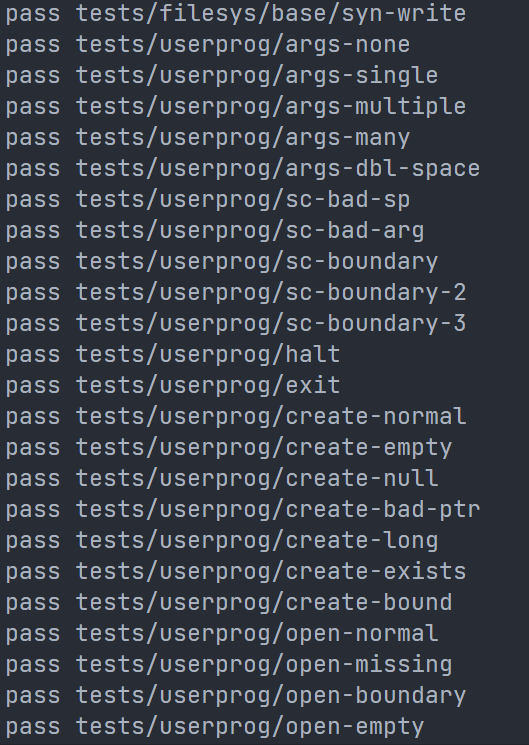
\includegraphics[width=0.4\textwidth]{img/2.png}}
  [1]     % 重点就在这,优先横向排列,自动换行
  \subfloat
  {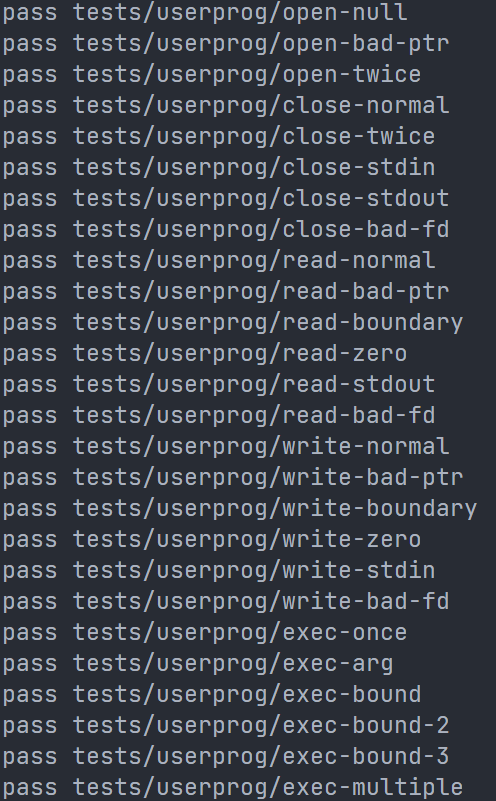
\includegraphics[width=0.4\textwidth]{img/3.png}}
  [2]
  \subfloat
  {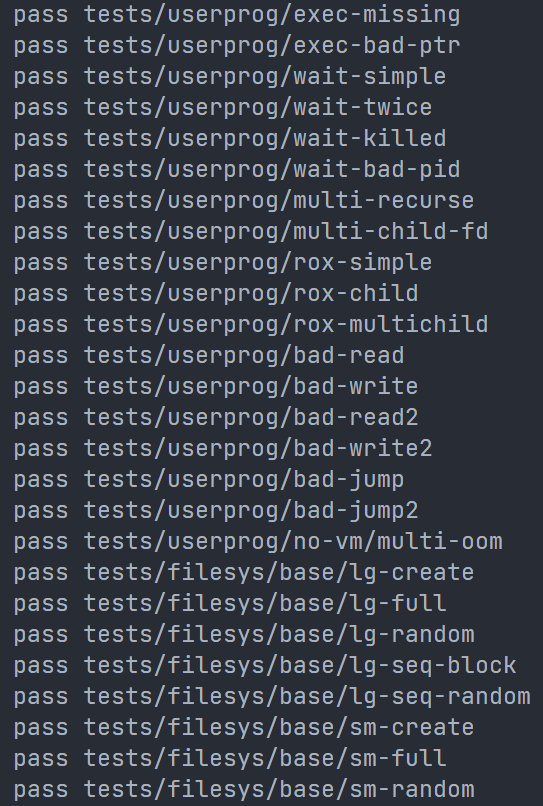
\includegraphics[width=0.4\textwidth]{img/4.png}}
  [3]
  \subfloat
  {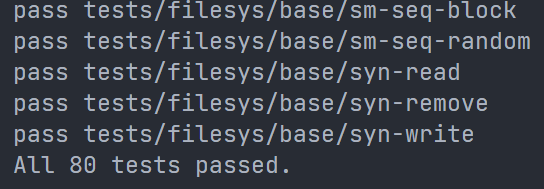
\includegraphics[width=0.4\textwidth]{img/5.png}}
  [4]
  \caption{实验的测试截图}
\end{figure}

具体实验分析可以参考上文。

\section{实验结果总结}

在本次实验中,我完成了参数传递和13个系统调用的实现,对操作系统进程管理、内存管理、文件系统管理有了更深入的了解。

\normalsize

\section{附录(源代码)}

见 \texttt{source-code-pintos-anon.tar.gz} 或 \texttt{source-code-pintos-anon.zip}。

也可以访问仓库 \url{https://github.com/llipengda/pintos-anon/tree/pdli-project2}。

\normalsize
\end{document}